\documentclass{article} % For LaTeX2e
\usepackage{iclr2027_conference,times}

% Optional math commands (standard notation package)
\input{math_commands.tex}

\usepackage{hyperref}
\usepackage{url}
\usepackage{booktabs}
\usepackage{graphicx}
\usepackage{amsmath,amssymb}
\usepackage{multirow}

\title{Emergent Selective Learning in Fast/Slow Learners:\\
Allocation-Level Selectivity of Consolidation\\ Without Any Selection Objective}

\author{Anonymous authors\\
Paper under double-blind review}

\begin{document}
\maketitle

\begin{abstract}
Selective learning---retaining some changes while discarding others---is usually treated as something an algorithm must explicitly implement (loss weighting, parameter gates, per-item replay). We ask whether it can instead \emph{emerge} from an unselective learning rule, and whether the emergent selectivity is functionally real. We study a minimal fast/slow learner on a fixed Transformer backbone: a fast weight $W_{\mathrm{fast}}$ integrates the learner's own gradient history (Adam-shaped, leaky), and at task boundaries an \emph{unselective} rule copies a scaled $W_{\mathrm{fast}}$ into the slow weights at a uniform scalar coefficient---no per-parameter gate, no success signal, no alignment objective. On a 6.59M Chinese character GPT with two curriculum histories (easy$\to$hard vs.\ hard$\to$easy) probed on a never-seen domain we find: (1) history-dependent future adaptation is causally tied to the fast-weight trace (swap control, $n{=}12$); (2) the pathway that transfers part of that trace into slow weights is the \emph{direct} fast$\to$slow write, not the architecture's explicitly designed success-gated eligibility trace $Q$, which is numerically ($\sim$0.4\% of write energy) and causally inert; and (3) the direct write's \textbf{coordinate allocation is functionally necessary}---keeping every write's energy identical but randomly permuting which coordinates receive it removes the entire effect ($n{=}12$, paired $t\approx5.5$; shuffled allocation $\approx$ no consolidation, and a misallocated write stays on the no-consolidation floor at every write strength we tried, while the benefit is graded rather than knife-edge over a $3\times$ range). Because the write is $\gamma W_{\mathrm{fast}}$ with a single scalar coefficient, ``where it writes'' is fully self-organized from the fast trace's own structure. We conclude that a minimal, unselective rule can exhibit \emph{emergent, allocation-level selective learning}, that this selectivity carries causal weight for future adaptation, and that it coexists with an explicit but non-functional selection mechanism. We report all claims with their evidence level and provide energy-matched controls throughout.
\end{abstract}

\section{Introduction}

\subsection{The question: does selectivity need to be designed?}

A learner with a memory faces a choice at every update: keep or discard. Machine learning usually makes this choice explicit---regularization that penalizes change to important weights \citep{kirkpatrick2017overcoming, zenke2017continual}, replay buffers that rehearse chosen items \citep{robins1995catastrophic, delange2021continual}, gated plasticity that opens or closes parameters \citep{miconi2019differentiable, beaulieu2020learning}, or curricula that choose what to learn next \citep{poirier2005effect, bell2022effect, li2025optimal}. Neuroscience likewise postulates specialized structures for selective retention \citep{mcclelland1995why, kumaran2016what}.

We ask a complementary, more mechanistic question:

\begin{quote}
If \emph{no} selection signal is ever computed---no per-parameter gate, no success weighting, no importance measure---can selectivity still emerge, and if it does, is it functionally real or an epiphenomenon?
\end{quote}

Selectivity is only meaningful if it has operational consequences. Our test is therefore causal: we must be able to \emph{destroy the allocation} while keeping everything else (total write energy, magnitudes) identical, and show the outcome changes.

\subsection{Why a fast/slow learner is the right object}

Fast/slow weight architectures \citep{hinton1987using, ba2016using} are the simplest systems in which ``what to consolidate'' is a well-defined choice: a fast store accumulates recent changes, and a slow store must decide what to accept. Modern revivals \citep{schlag2021linear, vonoswald2023transformers, behrouz2025titans} and parameter-efficient additive methods \citep{houlsby2019parameter, hu2022lora, he2022towards} make the same conceptual split. These systems typically ship with an explicit consolidation policy. We strip the policy to its minimum---an unselective scalar-copy---and ask whether selectivity re-appears on its own.

\subsection{The claim in one paragraph}

In a minimal DLA (\S\ref{sec:system}), two different curriculum histories produce different future adaptation on a never-seen domain, and this effect is carried by the fast-weight trace $W_{\mathrm{fast}}$ (\S\ref{sec:carrier}). Consolidation into the slow store happens through two pathways: a \emph{designed} one (a success-gated eligibility trace $Q$) and an \emph{unselective} one (direct copy of $W_{\mathrm{fast}}$). The designed pathway is inert; the unselective one carries the effect (\S\ref{sec:pathways}). Critically, the unselective pathway is \emph{selective in its allocation}: where it writes is dictated by the self-organized structure of $W_{\mathrm{fast}}$, and destroying that allocation (energy-matched within-matrix shuffle) removes the effect (\S\ref{sec:allocation}, $n{=}12$, paired $t\approx5.5$). We call this \textbf{emergent selective learning}, and we are careful to define its level (allocation of writes, not experience-level or success-gated selection).

\subsection{A causally instrumented setting, built on established fast/slow results}

The learner we use is not new to this paper, and we deliberately build on the fast/slow results established earlier in the project rather than re-deriving them:
\begin{itemize}
\item \textbf{Fast/slow separation protects consolidated memory}: in the same protocol, DLA matches a tuned AdamW on new-domain adaptation while slow-memory forgetting is $\approx$0 ($-0.4\%$), i.e.\ the fast/slow split does not trade memory for plasticity.
\item \textbf{$W_{\mathrm{fast}}$ is a causal carrier of history-dependent future adaptation}: replacing a hard$\to$easy learner's fast weights with an easy$\to$hard learner's degrades future adaptation on a never-seen domain ($n{=}12$, norm/shuffle/module controls, direction replicated on a second backbone).
\item \textbf{Rule parameters $\varphi$ and the success-gated eligibility trace $Q$ do not carry that effect}; and standard continual learners (AdamW, replay, EWC) in the same curriculum protocol are also history-sensitive, so history sensitivity is not unique to DLA---DLA is most robust after a difficult history.
\end{itemize}

These earlier findings are what make $W_{\mathrm{fast}}$, $Q$ and the slow store a \emph{causally instrumented} setting rather than a toy: the question below---whether selectivity can emerge with no selection objective---is asked about states whose causal roles are already mapped.

\subsection{Foundations we build on---and where we depart}

This paper is written on top of four strands of prior work (each maps to a claim we make), and its contribution is the gap at their intersection: \textbf{does the selectivity that continual-learning, plasticity and consolidation research usually \emph{injects} actually have to be injected?}

\textbf{(1) Theoretical root: why fast/slow stores and consolidation exist.} Complementary learning systems theory explains memory/learning trade-offs by a fast, instance-based store and a slow, generalising store with offline consolidation \citep{mcclelland1995why, kumaran2016what}. DLA is a minimal weight-space instantiation of that split (\S\ref{sec:learner}), and our result speaks back to CLS: consolidation that is functionally \emph{selective in its allocation} can arise without any gating/replay mechanism.

\textbf{(2) Structural twin: frozen-base additive updates.} Our effective weight $W_{\mathrm{eff}} = W_{\mathrm{slow}} + \mathrm{softplus}(P)\odot W_{\mathrm{fast}}$ is the same additive decomposition used by parameter-efficient transfer---adapters \citep{houlsby2019parameter} and LoRA \citep{hu2022lora}, unified in \citet{he2022towards}. DLA differs in that the additive pathway is a shared, within-lifetime developmental state rather than a per-task fine-tune. Because of this structural twin, our central question---\emph{whether ``where the additive update lands'' self-organizes and matters}---transfers directly to the LoRA/adapter setting in continual fine-tuning.

\textbf{(3) Plasticity motivation.} Plasticity is a fragile resource that ordinary continual training consumes \citep{dohare2024loss, lyle2022understanding, nikishin2022primacy}. DLA's per-parameter $P$ is one response to that literature. Our finding offers a complementary view: keeping \emph{beneficial structure in what is written to the slow store} may not require maintaining an explicit gate at all.

\textbf{(4) The nearest prior: task/curriculum ordering.} The order in which tasks are learned changes continual-learning outcomes, forgetting and consolidation of \emph{seen} tasks \citep{bell2022effect, li2025optimal, poirier2005effect, wang2022survey}. We ask a related but distinct question: does order change \emph{future adaptation to a never-seen domain}, and where inside the learner does the effect live? The difference is not cosmetic: because the test domain is never seen by either history, content-memory explanations of the order effect are excluded by design, which is what lets us localize the effect to $W_{\mathrm{fast}}$ and then to the \emph{allocation} of the fast$\to$slow write.

\emph{Position in one sentence:} existing work tells us history/order matters (4) and gives us the right architecture family (1, 2) and the warning that plasticity is fragile (3); we ask what happens when the selection machinery these strands normally provide is \emph{not} provided---and find that selectivity still emerges, at the level of write allocation, with causal force.

\section{System and definitions}
\label{sec:system}

\subsection{The learner (minimal DLA)}
\label{sec:learner}

We keep a standard Transformer backbone unchanged. Every wrapped weight matrix carries state:
\begin{equation}
W_{\mathrm{eff}} = W_{\mathrm{slow}} + \mathrm{softplus}(P)\odot W_{\mathrm{fast}}
\end{equation}

This additive decomposition is the structural twin of frozen-base parameter-efficient methods---adapters \citep{houlsby2019parameter} and LoRA \citep{hu2022lora, he2022towards}---with one difference that matters: here the additive pathway is a \emph{within-lifetime developmental state} shared across tasks and updated by the learner's own dynamics, not a separately fine-tuned module. $P$ is the per-parameter plasticity whose fragility under continual training is documented by loss-of-plasticity work \citep{dohare2024loss, lyle2022understanding, nikishin2022primacy}. The fast/slow split itself follows complementary learning systems theory \citep{mcclelland1995why, kumaran2016what}, and fast/slow co-design has engineering precedent in optimization and RLHF \citep{qi2024online} and modern memory architectures \citep{ba2016using, behrouz2025titans}.

Wake step (per batch): backprop gives $g = \mathrm{d}L/\mathrm{d}W_{\mathrm{eff}}$; Adam moments $m,v$ are updated; the fast trace moves by
\begin{equation}
\mathrm{d}w_t = -\eta_{\mathrm{fast}}\,\mathrm{softplus}(P_t)\odot \hat{a}_t - \lambda_{\mathrm{fast}}\,W_{\mathrm{fast},t},\qquad W_{\mathrm{fast},t+1} = W_{\mathrm{fast},t} + \mathrm{d}w_t
\end{equation}

$W_{\mathrm{fast}}$ is therefore a \emph{leaky integrator} (decay 0.02/step $\Rightarrow$ $\approx$50-step horizon $\approx$ one curriculum stage) of the learner's own Adam-shaped gradient history. $P$ is a per-parameter positive scale updated by a progress$\times$relevance rule. A designed consolidation trace is also maintained: $Q \leftarrow (1-\alpha)Q + \alpha\,(dw\cdot\mathrm{success})$, where \texttt{success} is a \textbf{single global scalar} derived from loss EMA---so the designed ``selection'' applies one coefficient to every parameter (this is deliberate; \S\ref{sec:levels} formalizes why it cannot select).

Sleep (task boundary): two write pathways into $W_{\mathrm{slow}}$:
\begin{equation}
W_{\mathrm{slow}} \leftarrow W_{\mathrm{slow}} + \beta Q + \gamma W_{\mathrm{fast}}
\end{equation}
\begin{equation}
W_{\mathrm{fast}} \leftarrow \delta\,W_{\mathrm{fast}},\qquad Q \leftarrow \rho\,Q,\qquad m,v \leftarrow 0
\end{equation}

The second term is the \textbf{unselective pathway}: every coordinate is copied with the same scalar $\gamma$. No objective, no gate, no importance weight---only $W_{\mathrm{fast}}$'s own structure decides, per coordinate, how much is written (the increment at coordinate $i$ is $\gamma W_{\mathrm{fast},i}$).

\subsection{Defining ``selectivity'' precisely}
\label{sec:levels}

\begin{table}[h]
\centering
\small
\begin{tabular}{@{}p{0.16\textwidth}p{0.62\textwidth}c@{}}
\toprule
level & definition & by design? \\
\midrule
step/global & one scalar decides keep-vs-discard for the whole update & yes (\texttt{success}) \\
parameter & different coefficients per parameter from a per-parameter signal & no \\
subspace & selection along learned/structured directions & no \\
\textbf{allocation} & unselective coefficient, but \emph{magnitude/sign per coordinate} varies & yes (emergent) \\
\bottomrule
\end{tabular}
\caption{The three levels at which ``selectivity'' can be defined, and which the system implements.}
\label{tab:levels}
\end{table}

Our paper's core construct is \textbf{allocation-level selectivity}: identical total energy and identical rule, but different coordinates receive different amounts because the source ($W_{\mathrm{fast}}$) is structured. Whether this allocation \emph{matters} is an empirical, causal question---answered by destroying it (energy-matched shuffle) while changing nothing else.

\subsection{Protocol and measurement}
\label{sec:protocol}

\begin{itemize}
\item Two histories on the same three curriculum domains (Wikipedia / SFT-QA / science Wikipedia) in opposite orders: easy$\to$hard (EH) and hard$\to$easy (HE).
\item Probe on a never-seen science slice D (40 steps, identical data/rule/budget/eval).
\item Metrics: gain@40 (relative ppl improvement), LE$_D$, T80. All causal/ablation claims use \textbf{within-seed, within-arm paired contrasts} (the raw EH/HE gap is seed-noisy).
\item Controls: cross-injection of state components; norm-matched / shuffled / module-localized swaps; consolidation ablations (Q-only / direct-only / none); and the energy-matched \textbf{allocation shuffle} (per-matrix random permutation of each sleep's $\gamma W_{\mathrm{fast}}$ increment).
\item Every claim is tagged by evidence level (causal / controlled / correlational / negative). No pre-registration; $n{=}10\to n{=}12$ transparent; no seed selection; no hyperparameter tuning for effect size.
\end{itemize}

\textbf{Aggregation provenance.} The consolidation/selectivity ablations were run \textbf{twice independently} on the same protocol, each $n{=}12$: (i) a first series assembled as $n{=}4$ (seeds 0--3) plus $n{=}8$ (seeds 4--11) extensions, and (ii) a later \textbf{unified batch} running all 12 seeds $\times$ 6 variants in one job, with same-protocol retention measured alongside. The two agree on every conclusion and on the core contrast (\texttt{direct}$-$\texttt{shufwrite} paired $t{=}{+}4.86$ and $t{=}{+}5.45$ respectively)---i.e.\ the central allocation result is \emph{independently replicated}. \textbf{All numbers quoted in this paper come from the unified batch}, except comparisons against the archived server \texttt{full} learners, which are labelled as such where they appear.

Backbone: 6.59M Chinese character GPT (6 layers, 8 heads, 256 dim, vocab 7280) pretrained on Chinese Wikipedia. Second setting (replication in direction only): 10.65M Shakespeare char GPT, $n{=}9$ (\S\ref{sec:second}).

\subsection{The mechanism chain, formalised}
\label{sec:chain}

We write the chain ``leaky integration $\to$ fast-weight structure $\to$ selective write-back $\to$ future adaptation'' as equations that match the code exactly; the evidence level of each arrow is stated in \S\ref{sec:discussion} and falsifiers are listed there.

\textbf{Link 1 --- leaky gradient integration (identity).} With teaching gradient $g_t = \nabla_{W_{\mathrm{eff}}} L_t$, Adam field $\hat{a}_t = \hat{m}_t/(\sqrt{\hat{v}_t}+\epsilon)$, gate $\varphi(P)=\mathrm{softplus}(P)$:
\begin{equation}
W_{\mathrm{fast},t+1} = (1-\lambda)\,W_{\mathrm{fast},t} - \eta\,\varphi(P_t)\odot \hat{a}_t
\end{equation}
\begin{equation}
\begin{aligned}
W_{\mathrm{fast},T} &= -\eta \sum_{k=0}^{T-1}(1-\lambda)^{T-1-k}\,\varphi(P_k)\odot \hat{a}_k \\
&= -\eta \sum_{k} \kappa(T,k)\,\hat{a}^{\varphi}_k,\qquad \kappa(T,k)=(1-\lambda)^{T-1-k}
\end{aligned}
\end{equation}
so the fast trace is the gated-Adam gradient field integrated with an exponential kernel of time constant $1/\lambda = 50$ steps ($\approx$ one 40-step curriculum stage). $\hat{a}$ is coordinate-normalised, so the integral preserves the sign/relative-magnitude structure of recent gradients and is invariant to per-coordinate scale.

\textbf{Link 2 --- fast-weight structure.} The history contrast between the two curricula is itself a difference of two such integrals,
\begin{equation}
\Delta_{\mathrm{hist}} = W_{\mathrm{fast}}^{\mathrm{HE}} - W_{\mathrm{fast}}^{\mathrm{EH}} = -\eta \sum_{k}\kappa(T,k)\left[\hat{a}^{\varphi}_k(\mathrm{HE}) - \hat{a}^{\varphi}_k(\mathrm{EH})\right]
\end{equation}
with no alignment term anywhere in the code. Empirically $\|\Delta_{\mathrm{hist}}\|$ and $\cos(W_{\mathrm{fast}}^{\mathrm{EH}}, W_{\mathrm{fast}}^{\mathrm{HE}})$ are indistinguishable from same-history cross-seed noise and PCA shows no dominant shared mode (\S\ref{sec:selforg}), so the structure is fine-grained and per-seed; the directional statistic $\rho = \cos(g_0, \Delta_{\mathrm{hist}})$ orders seeds by adaptation ($r{=}0.87$) but is correlational.

\textbf{Link 3 --- selective write-back.} The sleep operator writes two pathways (Eq.~3--4), whose allocation field is $A = \beta Q + \gamma W_{\mathrm{fast}}$. The direct term is \emph{unselective by rule} (a single scalar $\gamma$ multiplies every coordinate), so the placement of the write is entirely inherited from the self-organized trace: $A_i = \gamma W_{\mathrm{fast},i}$. We therefore define \textbf{allocation selectivity} operationally, by an energy-matched shuffle $A' = \Pi_{\pi} A$ with $\|A'\| = \|A\|$ exactly:
\begin{equation}
\text{selective} \iff \tau_{\mathrm{shuf}} := \mathbb{E}\!\left[G(\Phi_{\mathrm{shuf}})\right] - \mathbb{E}\!\left[G(\Phi_{\mathrm{direct}})\right] < 0\qquad\text{at fixed write energy}
\end{equation}
which holds ($\tau_{\mathrm{shuf}} = -0.0115$, paired $t{=}{-}5.45$, $n{=}12$) and is not reproduced by energy concentration (\texttt{uniformwrite}, \texttt{topwrite} both $\approx$ no-consolidation, \S\ref{sec:allocation}).

\textbf{Link 4 --- a first-order account of why placement matters.} For a small write $A$ onto $W_{\mathrm{slow}}$, the change of the future-task loss at the onset of adaptation is
\begin{equation}
\Delta L_D \approx \langle \nabla_{W_{\mathrm{slow}}} L_D,\, A\rangle + O(\|A\|^2)
\end{equation}
A write therefore helps exactly to the extent that it is \emph{aligned, coordinate by coordinate,} with the future-loss gradient field. Content-matched $A \propto W_{\mathrm{fast}}$ inherits partial alignment through Link 1; an energy-matched shuffle randomises the pairing, and $\mathbb{E}\langle \nabla L_D, \Pi A\rangle \approx 0$ unless the field carries a large constant component. This is the mathematical content of the shuffle control, and it also explains the modest absolute size of the effect (with $|\rho| \approx 0.02$, the first-order term is small).

\section{Results}

\subsection{History lives in the fast trace (carrier, causal)}
\label{sec:carrier}

Replacing a hard$\to$easy learner's $W_{\mathrm{fast}}$ with an easy$\to$hard learner's significantly degrades future adaptation on D: paired gain@40 $\Delta\approx-0.019$, 95\% CI $[-0.033,-0.005]$, sign $p{=}0.019$ (10/12 negative, $n{=}12$). Norm-matching does not rescue it ($d\approx-0.90$), within-matrix shuffling does not remove it ($d\approx-1.25$), and module-localized swaps implicate MLP ($d\approx-1.05$) and attention ($d\approx-1.06$) more than embedding ($d\approx-0.87$). The direction replicates on the Shakespeare backbone (\S\ref{sec:second}, $n{=}9$). Slow weights, plasticity and rule parameters transfer little alone (component decomposition). \emph{Level: causal (single small backbone, $n{=}12$, controls + partial replication).}

\textbf{Relation to task/curriculum-order results.} This mirrors, but differs from, the task-order results of continual learning \citep{bell2022effect, li2025optimal, poirier2005effect}: those measure how order changes \emph{performance or forgetting on the seen curriculum}. Here the probe domain D is never seen by either history, so the effect must ride on the learner's internal state rather than on stored content about D---which is what allows the further steps below (carrier localization, then allocation shuffle). Where those works propose curricula as a \emph{control} over outcomes, our claim is narrower and more mechanistic: the order effect is a \emph{state effect}, and that state effect is itself selective in where it consolidates.

\subsection{The directional trace is self-organized (no alignment objective exists)}
\label{sec:selforg}

A static code audit of the full wake/sleep/meta path confirms there is \textbf{no alignment operator anywhere} (no cosine/dot/objective between gradients and a history direction); directional content can only arise from $W_{\mathrm{fast}}$'s leaky integration of Adam-shaped gradients. Empirically, the per-seed alignment $\cos(g_0, \Delta W_{\mathrm{fast}})$ between the D-gradient and the same seed's history contrast predicts HE adaptation: $r{=}0.87$ (permutation $p\approx0.000$), leave-one-seed-out $r\in[0.81,0.91]$, survives FDR ($q\approx0.003$), survives norm-confound controls (partial $r\approx0.77$), and module-localizes to MLP/attention---the same modules implicated causally in \S\ref{sec:carrier}. \emph{Level: correlational, consistent with emergence; no direction-manipulation experiment.}

\subsection{Of two consolidation pathways, only the unselective one works}
\label{sec:pathways}

Measured on saved bodies: $\|Q\| \approx 0.002$ vs $\|W_{\mathrm{fast}}\| \approx 3.6$; the designed $Q$ write is $\approx$0.4\% of the direct write. Consolidation ablation on the HE arm ($n{=}12$, gain@40):

\begin{table}[h]
\centering
\small
\begin{tabular}{lcc}
\toprule
variant & mean (unified batch) & paired $t$ vs \texttt{direct} \\
\midrule
\texttt{direct} ($\gamma\cdot W_{\mathrm{fast}}$ only) & $+0.0140$ & --- \\
\texttt{nocons} (no write) & $+0.0027$ & $\mathbf{+7.36}$ \\
\texttt{qonly} ($\beta\cdot Q$ only; $n{=}4$) & $+0.0094$ & $\approx$ \texttt{nocons} \\
\bottomrule
\end{tabular}
\caption{Consolidation ablation. \texttt{direct} $\approx$ \texttt{full}: the same-protocol \texttt{full} learners from archived runs average $+0.0143$, a paired difference of $+0.0005$ ($t{=}{+}0.59$) against the Mac \texttt{direct} arm---an archived-vs-Mac comparison, not part of the unified batch and not re-derived here.}
\label{tab:pathways}
\end{table}

Removing consolidation drops the HE arm; the designed success-gated $Q$ pathway (which is the only ``selective'' mechanism in the code, and is global-scalar by construction) adds nothing on top of no-consolidation. \emph{Level: causal ($n{=}12$; $n{=}4$ for qonly).}

\subsection{The allocation of the unselective write is functionally necessary}
\label{sec:allocation}

Energy-matched allocation shuffle (\texttt{shufwrite}): identical to \texttt{direct} except each sleep's $\gamma W_{\mathrm{fast}}$ increment is randomly permuted \emph{within each matrix} before being added to $W_{\mathrm{slow}}$. Total energy, magnitudes, rule and coefficients are identical; only \emph{which coordinates} receive the write is destroyed.

HE arm, $n{=}12$ (unified batch): \texttt{shufwrite} mean $+0.0025$ vs \texttt{direct} $+0.0140$ $\to$ paired $\mathbf{t{=}{-}5.45}$ ($\tau_{\mathrm{shuf}}{=}{-}0.0115$); \texttt{shufwrite} $\approx$ \texttt{nocons} ($\Delta{=}{-}0.0002$ against the $+0.0027$ no-consolidation mean, i.e.\ indistinguishable given $sd\approx0.009$--$0.010$) $\ll$ \texttt{direct} ($t{=}{-}5.45$).

\begin{figure}[t]
\centering
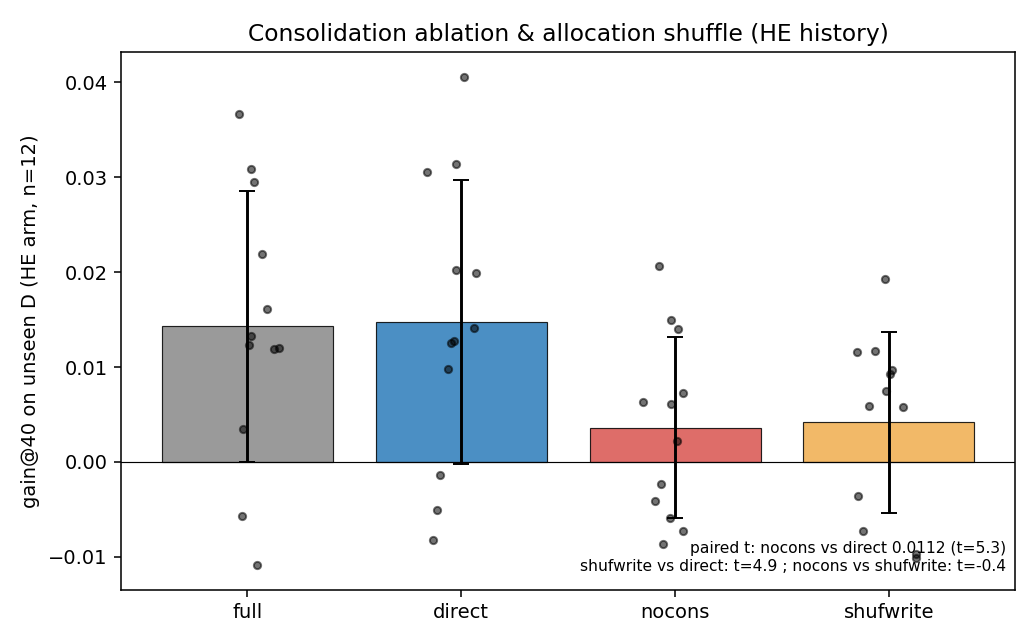
\includegraphics[width=0.95\textwidth]{figures/fig_audit_consolidation.png}
\caption{Consolidation ablation and allocation shuffle (HE arm, $n{=}12$). Destroying \emph{where} the write lands---while keeping its total energy exactly fixed---removes the effect entirely.}
\label{fig:consolidation}
\end{figure}

\textbf{Interpretation.} The write rule is scalar-uniform and unselective \emph{by rule}, yet its effect depends entirely on where the self-organized fast trace points it. The system therefore performs \textbf{allocation-level selection with no selection objective}---and the selection is not decorative: destroying it removes the effect. \emph{Level: causal ($n{=}12$; settings varied below).}

\begin{figure}[t]
\centering
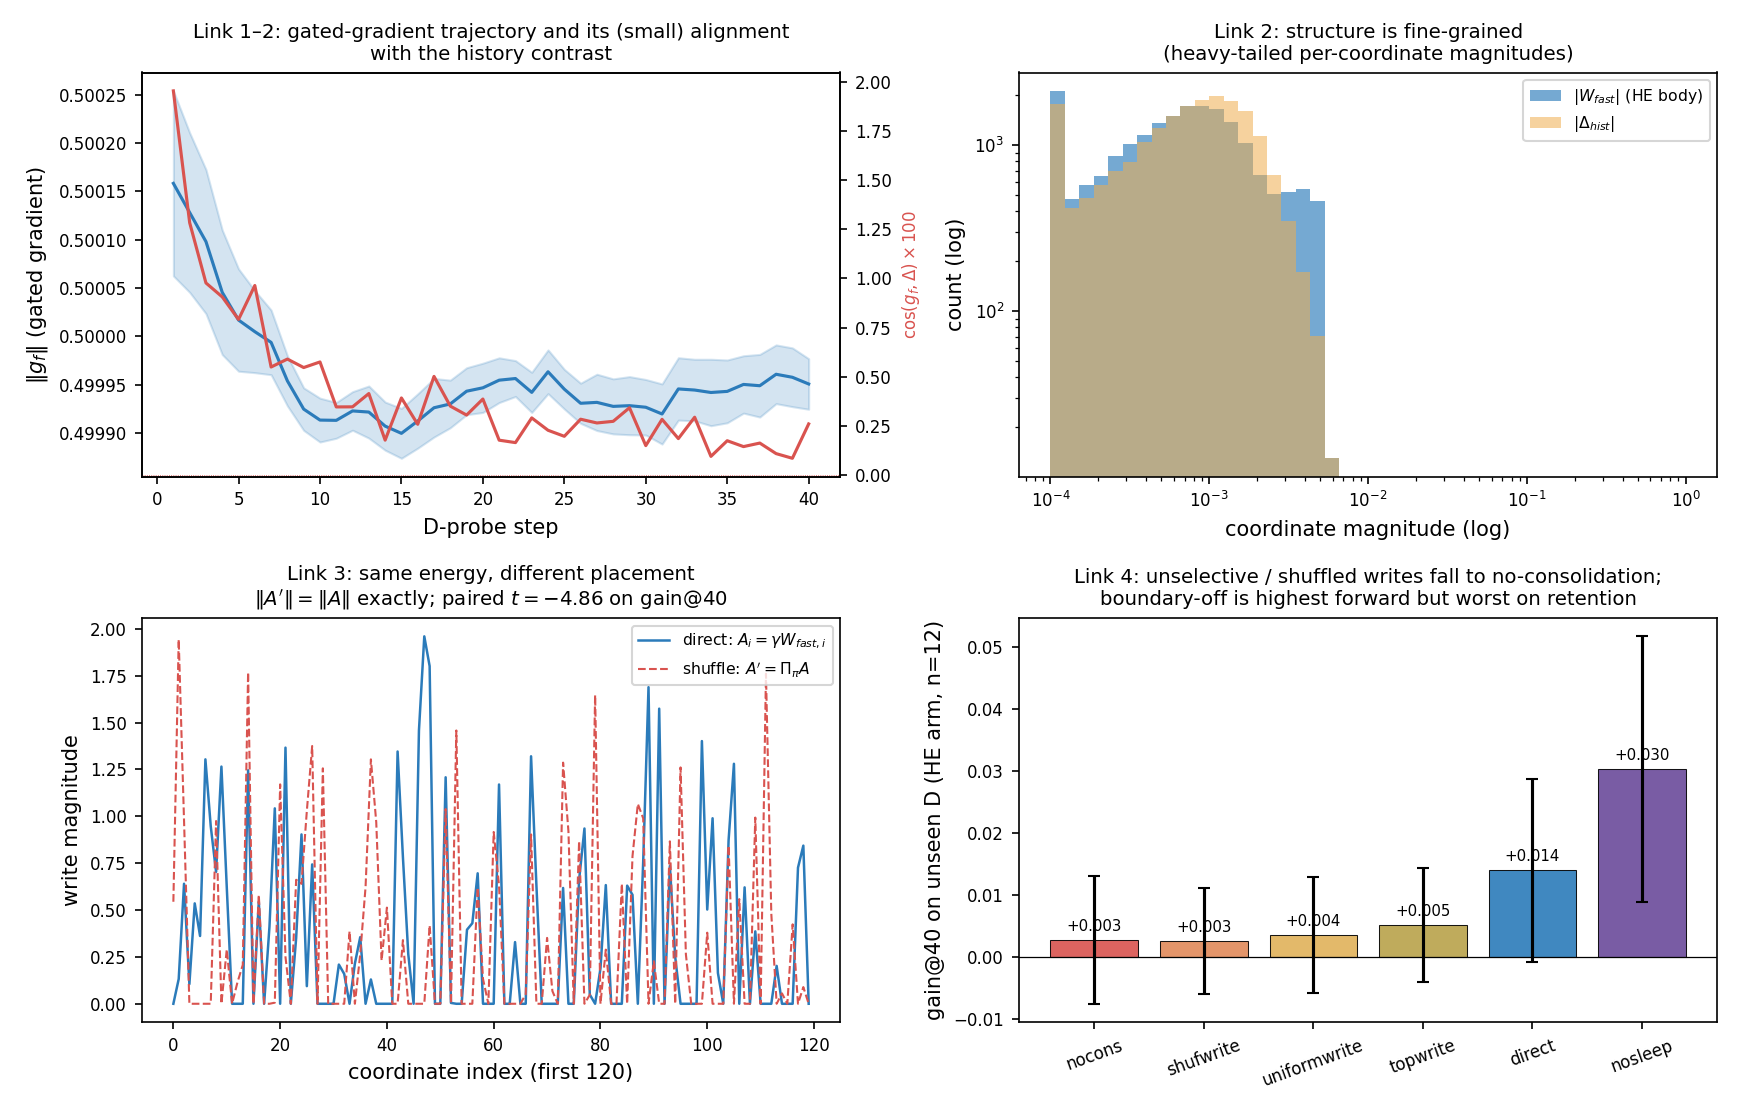
\includegraphics[width=0.95\textwidth]{figures/chain_empirical.png}
\caption{Mechanism chain, empirical panels ($n{=}12$ HE arm unless noted). Top-left: mean $\|g_f\|$ and $\cos(g_f,\Delta)\times100$ across the 40 D-probe steps. Top-right: per-coordinate magnitude distributions of $W_{\mathrm{fast}}$ and of the history contrast. Bottom-left: direct vs.\ energy-matched shuffled allocation. Bottom-right: gain@40 for the write-rule family---shuffled/uniform/top-concentrated writes fall to no-consolidation, boundary-off (\texttt{nosleep}) is highest forward but worst on retention.}
\label{fig:chain}
\end{figure}

\textbf{Is the effect an artifact of one write strength?} The result above is measured at the default setting ($\gamma_{\mathrm{scale}} = 1$). Since the claim rests on a single intervention at a single hyperparameter, the natural objection is that it could be a knife-edge artifact of that coefficient. We therefore swept the write strength over a $3\times$ range, re-running \textbf{both} arms at each setting under the same protocol, with the energy-matched shuffle applied at every setting (12 seeds each):

\begin{table}[h]
\centering
\small
\begin{tabular}{lcccc}
\toprule
$\gamma_{\mathrm{scale}}$ & \texttt{direct} & \texttt{shufwrite} & paired gap & $t$ \\
\midrule
0.5 & $+0.0059$ & $+0.0035$ & $+0.0024$ & $+1.82$ (n.s.) \\
\textbf{1.0} (default) & $+0.0140$ & $+0.0025$ & $\mathbf{+0.0115}$ & $\mathbf{+5.45}$ \\
1.5 & $+0.0241$ & $+0.0040$ & $\mathbf{+0.0201}$ & $\mathbf{+4.78}$ \\
\bottomrule
\end{tabular}
\caption{Write-strength robustness of allocation selectivity. The gap rises monotonically and both adjacent steps are individually significant (gap$(1.0)-$gap$(0.5)=+0.0091$, $t{=}{+}4.42$; gap$(1.5)-$gap$(1.0)=+0.0086$, $t{=}{+}3.57$), the direction the first-order account of \S\ref{sec:chain} predicts.}
\label{tab:dose}
\end{table}

A through-origin fit (slope $k{=}0.0123$) tracks the measured gaps for $\gamma \geq 1$, with the weakest setting falling \emph{below} the linear trend---a soft onset, not a threshold. A tail point at $\gamma_{\mathrm{scale}} = 0.05$ ($n{=}3$, underpowered) is consistent with this but supports no claim.

The sharper form of the same test: \textbf{the shuffled write never leaves the no-consolidation floor, at any write strength.} Relative to \texttt{nocons} ($+0.0027 \pm 0.0103$), \texttt{shufwrite} sits at $+0.0008$ / $-0.0002$ / $+0.0013$ for $\gamma_{\mathrm{scale}}$ = 0.5 / 1.0 / 1.5 (all n.s., $|dz| \leq 0.30$), while the coordinate-matched write climbs off that same floor ($+0.0032$ / $+0.0113$ / $+0.0215$ over \texttt{nocons}; $t = +2.38$ / $+7.36$ / $+6.58$). Adding 50\% more write energy to a misallocated write is simply wasted---what matters is \emph{where} the write lands, not how much is written.

\subsection{What does not happen (negative results, kept for honesty)}
\label{sec:negative}

\begin{itemize}
\item The EH arm shows no such effect in any variant (all $\approx 0$); the phenomenon is specific to the history/arm that carries the adaptation advantage.
\item The designed ``selective'' mechanism ($Q$, \texttt{success}) is numerically and causally inert (\S\ref{sec:pathways})---an explicit design coexisting with, but not causing, the emergent behavior.
\item More experience does not make learning faster: matched-difficulty $p{=}0.17$, cross-domain 20-seed $p{=}0.82$, physics near-transfer $d{=}{-}0.17$.
\item Macroscopic state geometry does not separate histories (norm/cosine at same-history cross-seed noise level; PCA PC1 $\approx$ 20\% variance).
\end{itemize}

\subsection{Same-protocol retention and the sleep boundary}
\label{sec:retention}

End-of-history ppl on the three seen curriculum domains, relative to birth ppl (more negative = better retained; $n{=}12$, HE arm):

\begin{table}[h]
\centering
\small
\begin{tabular}{lcc}
\toprule
variant & rel.\ forgetting mean$\pm$sd & paired vs \texttt{direct} ($t$) \\
\midrule
\texttt{direct} & $-0.0192 \pm 0.0083$ & --- \\
\texttt{nocons} & $-0.0152 \pm 0.0111$ & $+2.03$ (trend) \\
\texttt{nosleep} & $-0.0049 \pm 0.0079$ & $\mathbf{+10.26}$ \\
\bottomrule
\end{tabular}
\caption{Retention in the same protocol. The no-sleep individual is highest on the unseen-D probe ($+0.0303$ vs \texttt{direct} $+0.0140$, $t{=}{+}6.1$) but far worse at retention---the sleep boundary buys memory, not forward adaptation.}
\label{tab:retention}
\end{table}

\subsection{Ten-task continual learning}
\label{sec:t10}

Across a 10-domain sequence (\mbox{wiki$\to$qa$\to$physics}, \mbox{$\to$math$\to$computer$\to$biology}, \mbox{$\to$economics$\to$law$\to$history$\to$literature}), relative forgetting measured at the end of the sequence is: \texttt{direct} $-0.96\%\pm10.9$, \texttt{nocons} $-0.88\%\pm10.7$, \texttt{nosleep} $+0.79\%\pm11.0$ ($n{=}8$). Per-task heterogeneity dominates the aggregate; \texttt{direct} vs \texttt{nocons} is negligible except on one task ($-3.05\%$, $t{=}{-}4.56$), whereas \texttt{direct} vs \texttt{nosleep} is consistently negative ($t$ from $-2.65$ to $-13.6$). Averages over the first $k$ tasks stay within $\pm3\%$. We observe no accumulation or critical point within 10 tasks. \emph{Level: causal, but one backbone and no tuned baselines; longitudinal (forgetting vs.\ number of tasks learned) curves are unavailable because the protocol has no intermediate retention checkpoints.}

\subsection{Second-backbone replication}
\label{sec:second}

On a 10.65M Shakespeare char GPT with 3-chunk histories and 9 disjoint seeds: HE$+$EH $W_{\mathrm{fast}}$ swap $\Delta = -0.0673$ ($t{=}{-}7.13$); replacing the injected trace with an energy-matched shuffled variant gives $\Delta = -0.0721$ ($t{=}{-}7.60$); and HE$+$EH vs.\ shuffled-injection differ by $+0.0048$ ($t{=}{+}4.83$). The carrier direction therefore replicates on a different backbone and corpus. \emph{Level: causal (replication in direction only; small char model).}

\section{Discussion}
\label{sec:discussion}

\textbf{What we mean by ``emergent selective learning''.} Not ``the learner chooses experiences'' and not ``the learner computes importance''. Rather: a scalar-uniform consolidation rule, applied to a structured fast trace, produces per-coordinate differential retention that is \emph{causally required} for the history effect. Selectivity here is a property of the interaction between an unselective rule and a self-organized state, measurable only through interventions that destroy allocation (energy-matched shuffle).

\textbf{What the finding does and does not imply for design.} If allocation-selectivity emerges for free in minimal fast/slow learners, then ``selectivity'' need not be an added mechanism---and adding a \emph{global} scalar gate (like \texttt{success}) does not create it. Obtaining \emph{parameter-level or experience-level} selectivity would require genuinely new per-parameter/per-item signals and a channel with the same causal weight as the direct write (which currently dwarfs $Q$ by $\sim$250$\times$). This is directly relevant to plasticity-maintenance work \citep{dohare2024loss, lyle2022understanding, nikishin2022primacy} and to the design of ``growing'' learners.

\textbf{Limits.} One 6.59M backbone ($n{=}12$); raw EH/HE gap is seed-noisy (strong claims are within-seed paired); the directional-alignment result is correlational; retention is measured in the same protocol but the ten-task run has no tuned baselines; \texttt{qonly} was run at $n{=}4$; the write-strength sweep varies the direct-write coefficient only, and the separate sleep-decay axis was probed at just $n{=}6$ (indicative, not a result); second-backbone replication is $n{=}9$ with a shuffled-injection arm, but the second backbone is still a small char model with 3-chunk histories, and the selectivity/retention ablations were run on the Chinese backbone only. Scale is not yet tested: all results are at $\leq$11M parameters.

\textbf{Chain evidence levels and falsifiers.}

\begin{table}[h]
\centering
\small
\begin{tabular}{@{}cp{0.50\textwidth}p{0.17\textwidth}p{0.15\textwidth}@{}}
\toprule
link & statement & type & status \\
\midrule
1 & $W_{\mathrm{fast}}$ = gated-Adam gradient field, exponential kernel ($\tau\approx50$) & identity (code) & exact \\
2a & $\Delta_{\mathrm{hist}}$ is a difference of two such integrals; no alignment objective exists & static audit & established \\
2b & global geometry of $\Delta_{\mathrm{hist}}$ is indistinguishable from seed noise & measurement + null & established (negative) \\
2c & $\cos(g_0, \Delta_{\mathrm{hist}})$ orders seeds by adaptation ($r{=}0.87$) & correlational & supported, not causal \\
3 & direct write carries the effect; $Q$/success-gating inert & causal ($n{=}12$) & established \\
3$'$ & \textbf{allocation necessity}: energy-matched shuffle removes the effect & causal ($t{=}{-}5.45$) & \textbf{established (core)} \\
4a & forward adaptation: \texttt{direct} $\approx$ \texttt{full} & causal ($n{=}12$) & established \\
4b & retention: boundary protects old tasks; the write adds little relative retention & causal ($n{=}12$; 10-task $n{=}8$) & established \\
\bottomrule
\end{tabular}
\caption{The mechanism chain, statement by statement, with the type of evidence behind each.}
\label{tab:chain}
\end{table}

\textbf{Falsifiers we would accept:} (i) an explicit alignment objective found in the code (breaks 2a); (ii) the energy-matched shuffle losing significance at larger $n$ (breaks 3$'$) \emph{or} the direct$-$shuffled gap collapsing to zero outside the default write strength (which the $3\times$ sweep does \textbf{not} show---the gap grows monotonically there); (iii) $\tau_{\mathrm{shuf}} \approx \tau_{\mathrm{unif}} \approx \tau_{\mathrm{top}} \approx 0$ (placement irrelevant); (iv) direction manipulation ($\alpha\cdot\hat{\Delta}$ interpolation) failing to change adaptation (confines 2c to correlation); (v) retention surviving \texttt{nosleep} (moves the boundary claim to the write).

\section{Conclusion}

Selectivity can emerge where none is designed. In a minimal fast/slow learner with no alignment objective, no per-parameter gate, and a scalar-uniform consolidation rule, the learner's own gradient history shapes a fast trace whose coordinate structure determines where consolidation writes; keeping the total write energy identical but destroying that allocation removes the effect ($n{=}12$, paired $t\approx5.5$). The architecture's explicit, globally-gated ``selective'' pathway plays no measurable role. The lesson is twofold: emergent, allocation-level selective learning is real and causally potent in this setting; and designers should not assume that adding a selection \emph{signal} (especially a global one) is what creates selective behavior---or that selection needs to be added at all.

\subsection*{AI use statement}

An AI coding assistant was used to help implement experiment scripts, run the analysis pipeline, and draft and edit this manuscript. All experimental results were produced by the authors' own code and compute, were inspected by the authors, and the authors take full responsibility for all claims, analyses, and conclusions. No experimental result was generated or selected by a language model.

\subsection*{Reproducibility statement}

Code and per-seed results are provided as anonymized supplementary material. The protocol, hyperparameters, per-seed data and commit hashes are recorded for every claim. Mechanism-audit runs used a parity-validated harness (Apple M2 CPU; mean $|\Delta\mathrm{ppl}| \approx 0.24$ vs.\ archived server runs). All consolidation/selectivity numbers are quoted from one unified batch (12 seeds $\times$ 6 variants, single job), with an independent earlier series ($n{=}4+n{=}8$) retained as a replication of the same contrasts; the aggregation provenance of every quoted number is stated in \S\ref{sec:protocol}.

\bibliography{references}
\bibliographystyle{iclr2027_conference}

\end{document}
